\section{Referencial teórico}
\label{sec:referencialTeorico}
% Os principais conceitos aos quais os trabalho está relacionado. Por exemplo, apresentar os conceitos de Aprendizado de Máquina e métodos relacionados.
% As principais técnicas e métodos nos quais o trabalho se apoia (referências)

Antes de tratar sobre as definições mais específicas que este trabalho vai utilizar, gostaria de trazer uma definição mais geral em que o problema está incluído. Podemos compreender Sistemas de Informação como sistemas, sejam eles manuais ou automatizados, inter-relacionados que atuam armazenando, processando e transmitindo dados que representam informações para as partes interessadas (\textit{stakeholders}). De forma mais geral, esses sistemas "\textit{atuam em conjunto para o cumprimento de uma tarefa ou um objetivo}" \cite{turban2009business}. O grupo básico de operações de um Sistema de Informação é constituído pelas entradas, pelo processamento e pelas saídas (Figura \ref{fig:operacoesBasicaSistemas}). A entrada é o conjunto de dados que será usado pelo sistema, o processamento é composto pela transformações e combinações que os dados de entradas serão submetidos e, por fim, a saída é o produto obtido por meio do processamento dos dados de entrada. Em alguns casos, o sistema pode ser retroalimentado (\textit{feedback}), fazendo com que os dados de saída sejam manipulados como dados de entrada em uma nova execução. Neste processo, também é comum que ocorra o armazenamento dos dados de entrada e de saída para serem utilizados posteriormente, como pode ser visto na Figura \ref{fig:operacoesBasicaSistemas}.

\begin{figure}[ht]
\centering
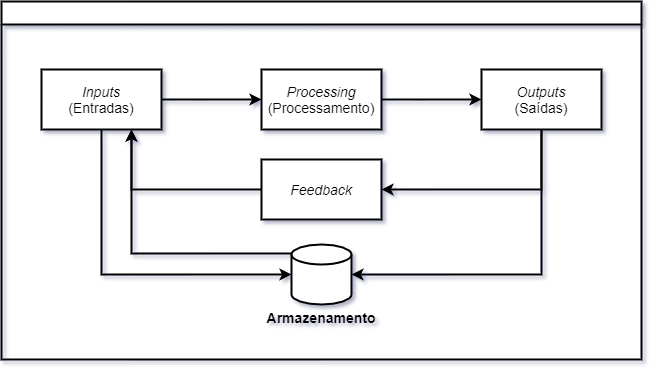
\includegraphics[width=1\textwidth]{imagens/operacoes-basicas-sistema-informacao.png}
\caption{Operações básicas de um Sitema de Informação.}
\label{fig:operacoesBasicaSistemas}
\end{figure}

% TODO falar sobre informação e dados https://integrada.minhabiblioteca.com.br/reader/books/9786556901916/pageid/17

